% Graphic for TeX using PGF
% Title: /home/di3go/workspace/t02-core-musa/doc/architecture/pictures/diagrams/registers_bank.dia
% Creator: Dia v0.97.3
% CreationDate: Wed Dec 17 00:36:05 2014
% For: di3go
% \usepackage{tikz}
% The following commands are not supported in PSTricks at present
% We define them conditionally, so when they are implemented,
% this pgf file will use them.
\ifx\du\undefined
  \newlength{\du}
\fi
\setlength{\du}{15\unitlength}
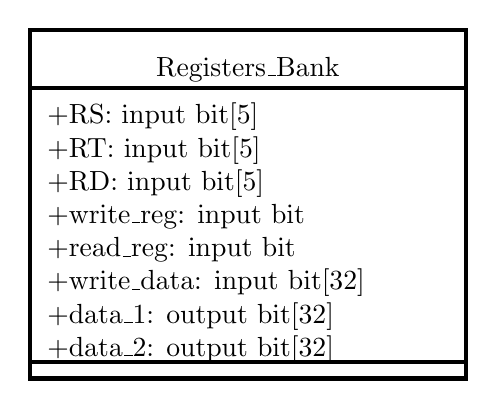
\begin{tikzpicture}
\pgftransformxscale{1.000000}
\pgftransformyscale{-1.000000}
\definecolor{dialinecolor}{rgb}{0.000000, 0.000000, 0.000000}
\pgfsetstrokecolor{dialinecolor}
\definecolor{dialinecolor}{rgb}{1.000000, 1.000000, 1.000000}
\pgfsetfillcolor{dialinecolor}
\pgfsetlinewidth{0.100000\du}
\pgfsetdash{}{0pt}
\definecolor{dialinecolor}{rgb}{1.000000, 1.000000, 1.000000}
\pgfsetfillcolor{dialinecolor}
\fill (18.050000\du,1.100000\du)--(18.050000\du,2.500000\du)--(28.560000\du,2.500000\du)--(28.560000\du,1.100000\du)--cycle;
\definecolor{dialinecolor}{rgb}{0.000000, 0.000000, 0.000000}
\pgfsetstrokecolor{dialinecolor}
\draw (18.050000\du,1.100000\du)--(18.050000\du,2.500000\du)--(28.560000\du,2.500000\du)--(28.560000\du,1.100000\du)--cycle;
% setfont left to latex
\definecolor{dialinecolor}{rgb}{0.000000, 0.000000, 0.000000}
\pgfsetstrokecolor{dialinecolor}
\node at (23.305000\du,2.050000\du){Registers\_Bank};
\definecolor{dialinecolor}{rgb}{1.000000, 1.000000, 1.000000}
\pgfsetfillcolor{dialinecolor}
\fill (18.050000\du,2.500000\du)--(18.050000\du,9.100000\du)--(28.560000\du,9.100000\du)--(28.560000\du,2.500000\du)--cycle;
\definecolor{dialinecolor}{rgb}{0.000000, 0.000000, 0.000000}
\pgfsetstrokecolor{dialinecolor}
\draw (18.050000\du,2.500000\du)--(18.050000\du,9.100000\du)--(28.560000\du,9.100000\du)--(28.560000\du,2.500000\du)--cycle;
% setfont left to latex
\definecolor{dialinecolor}{rgb}{0.000000, 0.000000, 0.000000}
\pgfsetstrokecolor{dialinecolor}
\node[anchor=west] at (18.200000\du,3.200000\du){+RS: input bit\ensuremath{[}5\ensuremath{]}};
% setfont left to latex
\definecolor{dialinecolor}{rgb}{0.000000, 0.000000, 0.000000}
\pgfsetstrokecolor{dialinecolor}
\node[anchor=west] at (18.200000\du,4.000000\du){+RT: input bit\ensuremath{[}5\ensuremath{]}};
% setfont left to latex
\definecolor{dialinecolor}{rgb}{0.000000, 0.000000, 0.000000}
\pgfsetstrokecolor{dialinecolor}
\node[anchor=west] at (18.200000\du,4.800000\du){+RD: input bit\ensuremath{[}5\ensuremath{]}};
% setfont left to latex
\definecolor{dialinecolor}{rgb}{0.000000, 0.000000, 0.000000}
\pgfsetstrokecolor{dialinecolor}
\node[anchor=west] at (18.200000\du,5.600000\du){+write\_reg: input bit};
% setfont left to latex
\definecolor{dialinecolor}{rgb}{0.000000, 0.000000, 0.000000}
\pgfsetstrokecolor{dialinecolor}
\node[anchor=west] at (18.200000\du,6.400000\du){+read\_reg: input bit};
% setfont left to latex
\definecolor{dialinecolor}{rgb}{0.000000, 0.000000, 0.000000}
\pgfsetstrokecolor{dialinecolor}
\node[anchor=west] at (18.200000\du,7.200000\du){+write\_data: input bit\ensuremath{[}32\ensuremath{]}};
% setfont left to latex
\definecolor{dialinecolor}{rgb}{0.000000, 0.000000, 0.000000}
\pgfsetstrokecolor{dialinecolor}
\node[anchor=west] at (18.200000\du,8.000000\du){+data\_1: output bit\ensuremath{[}32\ensuremath{]}};
% setfont left to latex
\definecolor{dialinecolor}{rgb}{0.000000, 0.000000, 0.000000}
\pgfsetstrokecolor{dialinecolor}
\node[anchor=west] at (18.200000\du,8.800000\du){+data\_2: output bit\ensuremath{[}32\ensuremath{]}};
\definecolor{dialinecolor}{rgb}{1.000000, 1.000000, 1.000000}
\pgfsetfillcolor{dialinecolor}
\fill (18.050000\du,9.100000\du)--(18.050000\du,9.500000\du)--(28.560000\du,9.500000\du)--(28.560000\du,9.100000\du)--cycle;
\definecolor{dialinecolor}{rgb}{0.000000, 0.000000, 0.000000}
\pgfsetstrokecolor{dialinecolor}
\draw (18.050000\du,9.100000\du)--(18.050000\du,9.500000\du)--(28.560000\du,9.500000\du)--(28.560000\du,9.100000\du)--cycle;
\end{tikzpicture}
